\chapter{Systembeskrivelse}
Dette kapitel indeholder en introducerende beskrivelse af den udviklede prototype, herunder brugergrænsefladen og dens fysiske opbygning. Herudover indeholder kapitlet en beskrivelse af sorteringsprocessen og generelle egenskaber for de langerhanske øer.

Figur \ref{fig:system} viser den overordnede opbygning af systemet. Grundlæggende består systemet af en beholder indeholdene opløsningen med langerhanske øer. Opløsningen pumpes herefter ved hjælp af en pumpe i gennem en slange, hvor et kamera detektere om en ø passere eller ej. Hvis en ø detekteres åbner systemet en ventil for at frasortere øen fra resten af opløsningen. Systemet består af et software program udviklet i Matlab, hvor operatøren har mulighed for at interagere med systemet. Her er selve logikken og signalbehandlingen i form af billedprocessering implementeret. Programmet giver signal til en Microcontroller (Arduino platform), som håndterer styring af hardware komponenterne.

\begin{figure}[H]
	\centering
	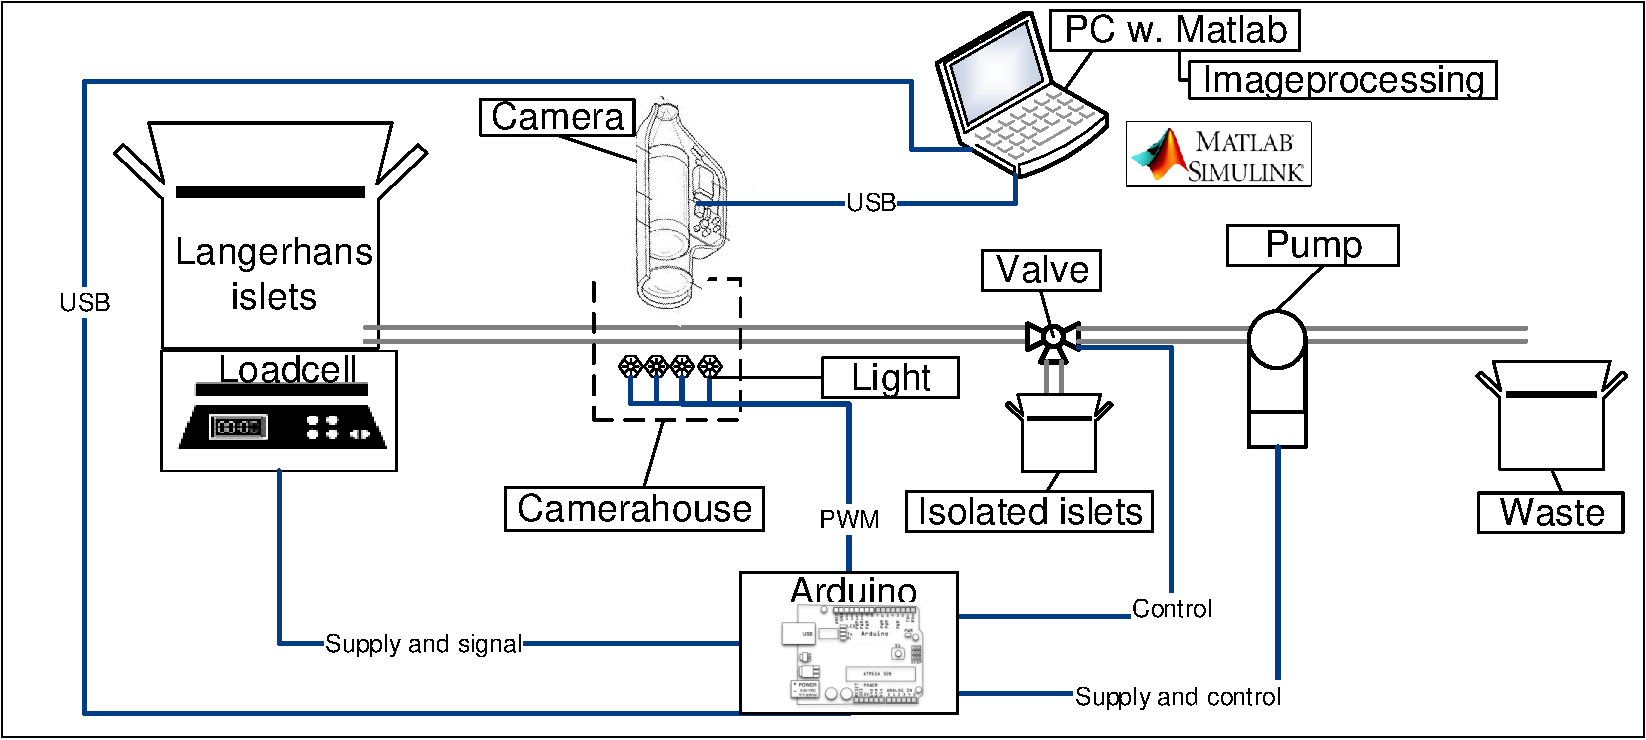
\includegraphics[width=1\textwidth]{billeder/DMTS.pdf}
	\caption{Figuren viser den overordnede opbygning af systemet}
	\label{fig:system}
\end{figure}
Beskrivelse 

Figur over systemet

Billeder af det færdige system

Skal brugergrænseflade og hardware først komme i resultat afsnittet ?? 
\section{Brugergrænseflade}
Billeder og beskrivelser

\section{Hardware}


\section{Sorteringsproces}
Dette afsnit beskriver hvordan sorteringsprocessen foregår, samt generelle egenskaber for opløsningen med langerhanske øer. 

\subsection{Sorteringsproces}
Isoleringsbeskrivelse 

Med trinvis figur evt? 
\subsection{Langerhanske øer}
Den endelige opløsning består udover de langerhanske øer af "ekstra væv" \fxnote{Hvad er det?} og fysiologisk saltvand. \fxnote{er dette rigtigt}.

Figur \fxnote{vi skal ha taget nogle billeder fra petriskål}, viser hvordan opløsningen ser ud. På billedet er en del af opløsningen hældt i en petriskål.
 
Billeder fra petriskål

En petriskål på 10 ml vil typisk indeholde mellem 30 og 50 øer. Til et batch på 250 øer anvnedes typisk 5-6 mus. Den samlede mængde opløsningsvæske i sådan et batch er 250 ml.. \fxnote{Vi skal lige ha rettet nogle af de her tal ;-)}
